%%%%%%%%%%%%%%%%%%%%% introduction.tex %%%%%%%%%%%%%%%%%%%%%%%%%%%%%%%%%
%
% Introduction chapter
%
%%%%%%%%%%%%%%%%%%%%%%%% Springer-Verlag %%%%%%%%%%%%%%%%%%%%%%%%%%

\chapter{Introducão}
\label{introduction} % Always give a unique label
% use \chaptermark{}
% to alter or adjust the chapter heading in the running head

Programação em lógica com restrições é uma junção de dois paradigmas: solução de restrições e programação em lógica. Esta combinação permite uma concepção mais expressiva e flexível — e em alguns casos mais eficiente - de problemas lógicos.

\section{Motivação}
\label{sec:1}
% Always give a unique label
% and use \ref{<label>} for cross-references
% and \cite{<label>} for bibliographic references
% use \sectionmark{}
% to alter or adjust the section heading in the running head
A motivação deste trabalho incidiu na compreensão de um paradigma de programação que já nos é familiar, envolvendo uma nova componente de restrições; resolver problemas lógicos com restrições de uma forma geral, tendo a possibilidade de os refinar e otimizar para uma solução particular.

\section{Objectivos}
\label{sec:2}
Resolver a versão original do jogo Turn12 recorrendo a restrições; gerar cubos com um número de dígitos variável, e avaliar se estes têm solução ou não segundo as restrições definidas.

\section{Descrição do problema}
\label{sec:3}
O problema centra-se num cubo em que cada face contém dígitos numerados de 3 a 9, aleatoriamente. Na junção das arestas de cada face, a soma dos dois dígitos que se encontram deverá ser igual a 12.

A solução original (Fig. 2.1) com 24 dígitos por face é única.

A resolução que apresentamos contempla dígitos ilimitados, e uma vez que não existe qualquer padrão associado à sequência de dígitos no problema original, estes são gerados aleatóriamente e não é garantida a unicidade de solução.

No entanto, para valores demasiado elevados (superiores a 60 por face), as limitações de computação começaram-se a sentir e encontrar uma solução em tempo útil não foi possível, por limitações de Hardware.

%Figura cubo
\begin{figure}[h!]
\begin{center}
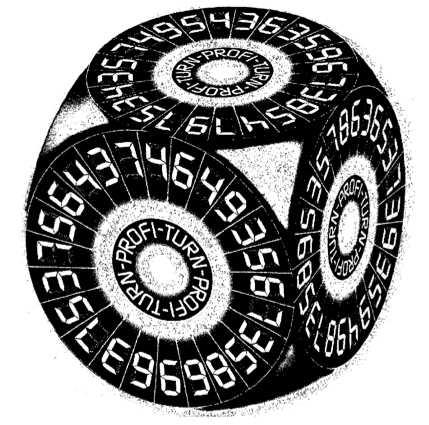
\includegraphics[scale=0.4]{turn12.png}
\caption{Problema original}
\label{fig:1}
\end{center}
\end{figure}

%
